%Type of document
\documentclass[a4paper, 12pt]{report}

%For easy management of document margins and the document page size
\usepackage[right=3.5cm,left=3.5cm,top=3.5cm,bottom=3.5cm]{geometry}

%Allows to insert graphic files within a document
\usepackage{graphicx}

%Sup­ports com­pressed, sorted lists of nu­mer­i­cal ci­ta­tions, and also deals with var­i­ous punc­tu­a­tion and %other is­sues of rep­re­sen­ta­tion, in­clud­ing com­pre­hen­sive man­age­ment of break points
\usepackage{cite}

%It gives LaTeX the possibility to manage links within the document or to any URL when you compile in PDF
\usepackage{hyperref}

%To choose the font encoding of the output text
\usepackage[T1]{fontenc}

%To choose the encoding of the input text
%Consente di usare le lettere accentate
\usepackage[latin1]{inputenc}

%It provides the internationalization of LaTeX. It has to be loaded in any document, and you have to give %as an option the main language you are going to use in the document
\usepackage[english]{babel}

%Allows to write algorithms
\usepackage{algorithm}
\usepackage{algpseudocode}

\normalfont
%Forza LaTeX ad una spaziatura uniforme, invece di lasciare più spazio
%alla fine dei punti fermi come da convenzione inglese
\frenchspacing
%Modifica della spaziatura interlineare
\linespread{1.3}

%Inizia il documento
\begin{document}

%Creazione di un frontespizio personalizzato
\begin{titlepage}

\begin{center}
\Large
\textbf{POLYTECHNIC UNIVERSITY OF MILAN} \\
\Large
School of Industrial and Information Engineering \\
Computer Science and Engineering
\end{center}

\addvspace{0.8cm}
%PER INSERIRE IMMAGINE
\begin{figure}[h]
\begin{center}

\includegraphics[width=3cm]{cpt/img/polimi}
\end{center}
\end{figure}

\addvspace{0.1cm}
\begin{center}
\LARGE

\textbf{Project of Software Engineering 2: MyTaxi Service \\
Design Document}

\end{center}

\addvspace{0.5cm}
\Large
\begin{center}
\begin{tabular}{p{1\textwidth}p{0.3\textwidth}}
Course Professor: Prof. Elisabetta DI NITTO \\
\end{tabular}
\end{center}

\addvspace{0.6cm}
\Large
\begin{center}
\begin{tabular}{p{0.6\textwidth}p{0.6\textwidth}}
& Authors: \\
& Mattia 	CRIPPA		854126\\
& Francesca GALLUZZI	788328\\
& Marco 	LATTARULO	841399
\end{tabular}
\end{center}

\vfill
\Large
\begin{center}
Academic Year 2015--2016
\end{center}
\end{titlepage}

\clearpage

\tableofcontents
\clearpage

\listoffigures
\clearpage

\listofalgorithms
\addtocontents{loa}{\def\string\figurename{Algorithm}}
\clearpage

\chapter{Introduction}
\clearpage

\chapter{Architectural Design} \label{chap2}

\section{Overview}

\section{High Level Components and their Interaction}

\section{Component View}

\section{Deployment View}

\section{Runtime View}

\section{Component Interfaces}

\section{Selected Architectural Styles and Patterns}

\section{Other Design Decisions}
\clearpage

\chapter{Algorithm Design} \label{chap3}
\subsubsection{Queue Management:}
It?s possible to create a queue implementing the Java Interface Queue, which is a collection designed for holdings elements prior to processing. Besides basic Collection operations, queues provide additional insertion, extraction, and inspection operations. Queues typically order elements in a FIFO (first-in-first-out) manner. The \textit{head} of the queue is that element which would be removed by a call to \textbf{remove()} or \textbf{poll()}. In a FIFO queue, all new elements are inserted at the \textit{tail} of the queue.
This Interface provides some methods to manage the queue:
\begin{itemize}
	\item \textbf{add(e)} $\rightarrow$ Method that allow to insert a new element e in the queue
	\item \textbf{remove()} and \textbf{poll()} $\rightarrow$ Methods that remove and return the head of the queue. Methods differ only in their behavior when the queue is empty: the remove() method throws an exception, while the poll() method returns null.
	\item \textbf{element()} and \textbf{peek()} $\rightarrow$ Methods that return, but do not remove, the head of the queue.
\end{itemize}

\subsubsection{Research of a Taxi Driver in the queue:}
The system uses a FIFO queue to manage the requests to the taxi drivers. It will use the method element() in order to extract without removing the first taxi driver of the queue and it will send the request to him. If the first taxi driver accepts the request, this will be assigned to him and he will be dequeued, otherwise he will be dequeued and the system will use the new first element of the queue to detect the new taxi driver who will receive the request, and so on until a taxi driver accepts the request.

\begin{algorithm}[H]
\caption{Research of a Taxi Driver}
\begin{algorithmic}[1]
\Procedure{SearchTaxiDriver}{$Q$}
\If{$(Q.head == Q.tail)$}\Comment{Queue is empty}
	\Else
	\For{$i:= 0$ \textbf{to} $Q.lenght$}
		\State $x \gets Dequeue(Q)$\Comment{Classical operation for managing the extraction of an element from the Queue}
		\State $acceptance \gets Call(x)$\Comment{Function that represent the call that the system makes to the driver in order to propose a ride. It \textbf{returns true} if the taxi driver accepts the call and is willing to make the ride, otherwise \textbf{returns false} if the taxi driver declines the call}
		\If{$(acceptance == true)$}
			\State $\textbf{return} \: x$
		\Else
			\State $Enqueue(Q, x)$\Comment{Classical operation for managing the insertion of an element from the Queue}
		\EndIf
	\EndFor
\EndIf
\EndProcedure
\end{algorithmic}
\end{algorithm}

\subsubsection{Shared Ride Management:}
This is the algorithm that is responsible to manage the Shared Rides. Here there are some general information about the algorithm: \\
There is one sharing list per every taxi area ordered by the starting time of the ride. Match between elements of the list is done under a time window of 10 minutes after the selected starting time (for reservation) and after the moment of the call (for request).When is time to start assigning a driver to the request/reservation and start the ride, the system deletes the corresponding element from the list (is always the head of the list because of the ordering). There is also a buffer (Figure \ref{fig:buff}) to make sequential the adding of new requests/reservations to the list and avoid conflicts.\\
The flowchart diagram in Figure \ref{fig:genalg} represent the generic algorithm which describes how the system manage the functionality of "Ride Sharing".

\begin{figure}[htbp]
\centering
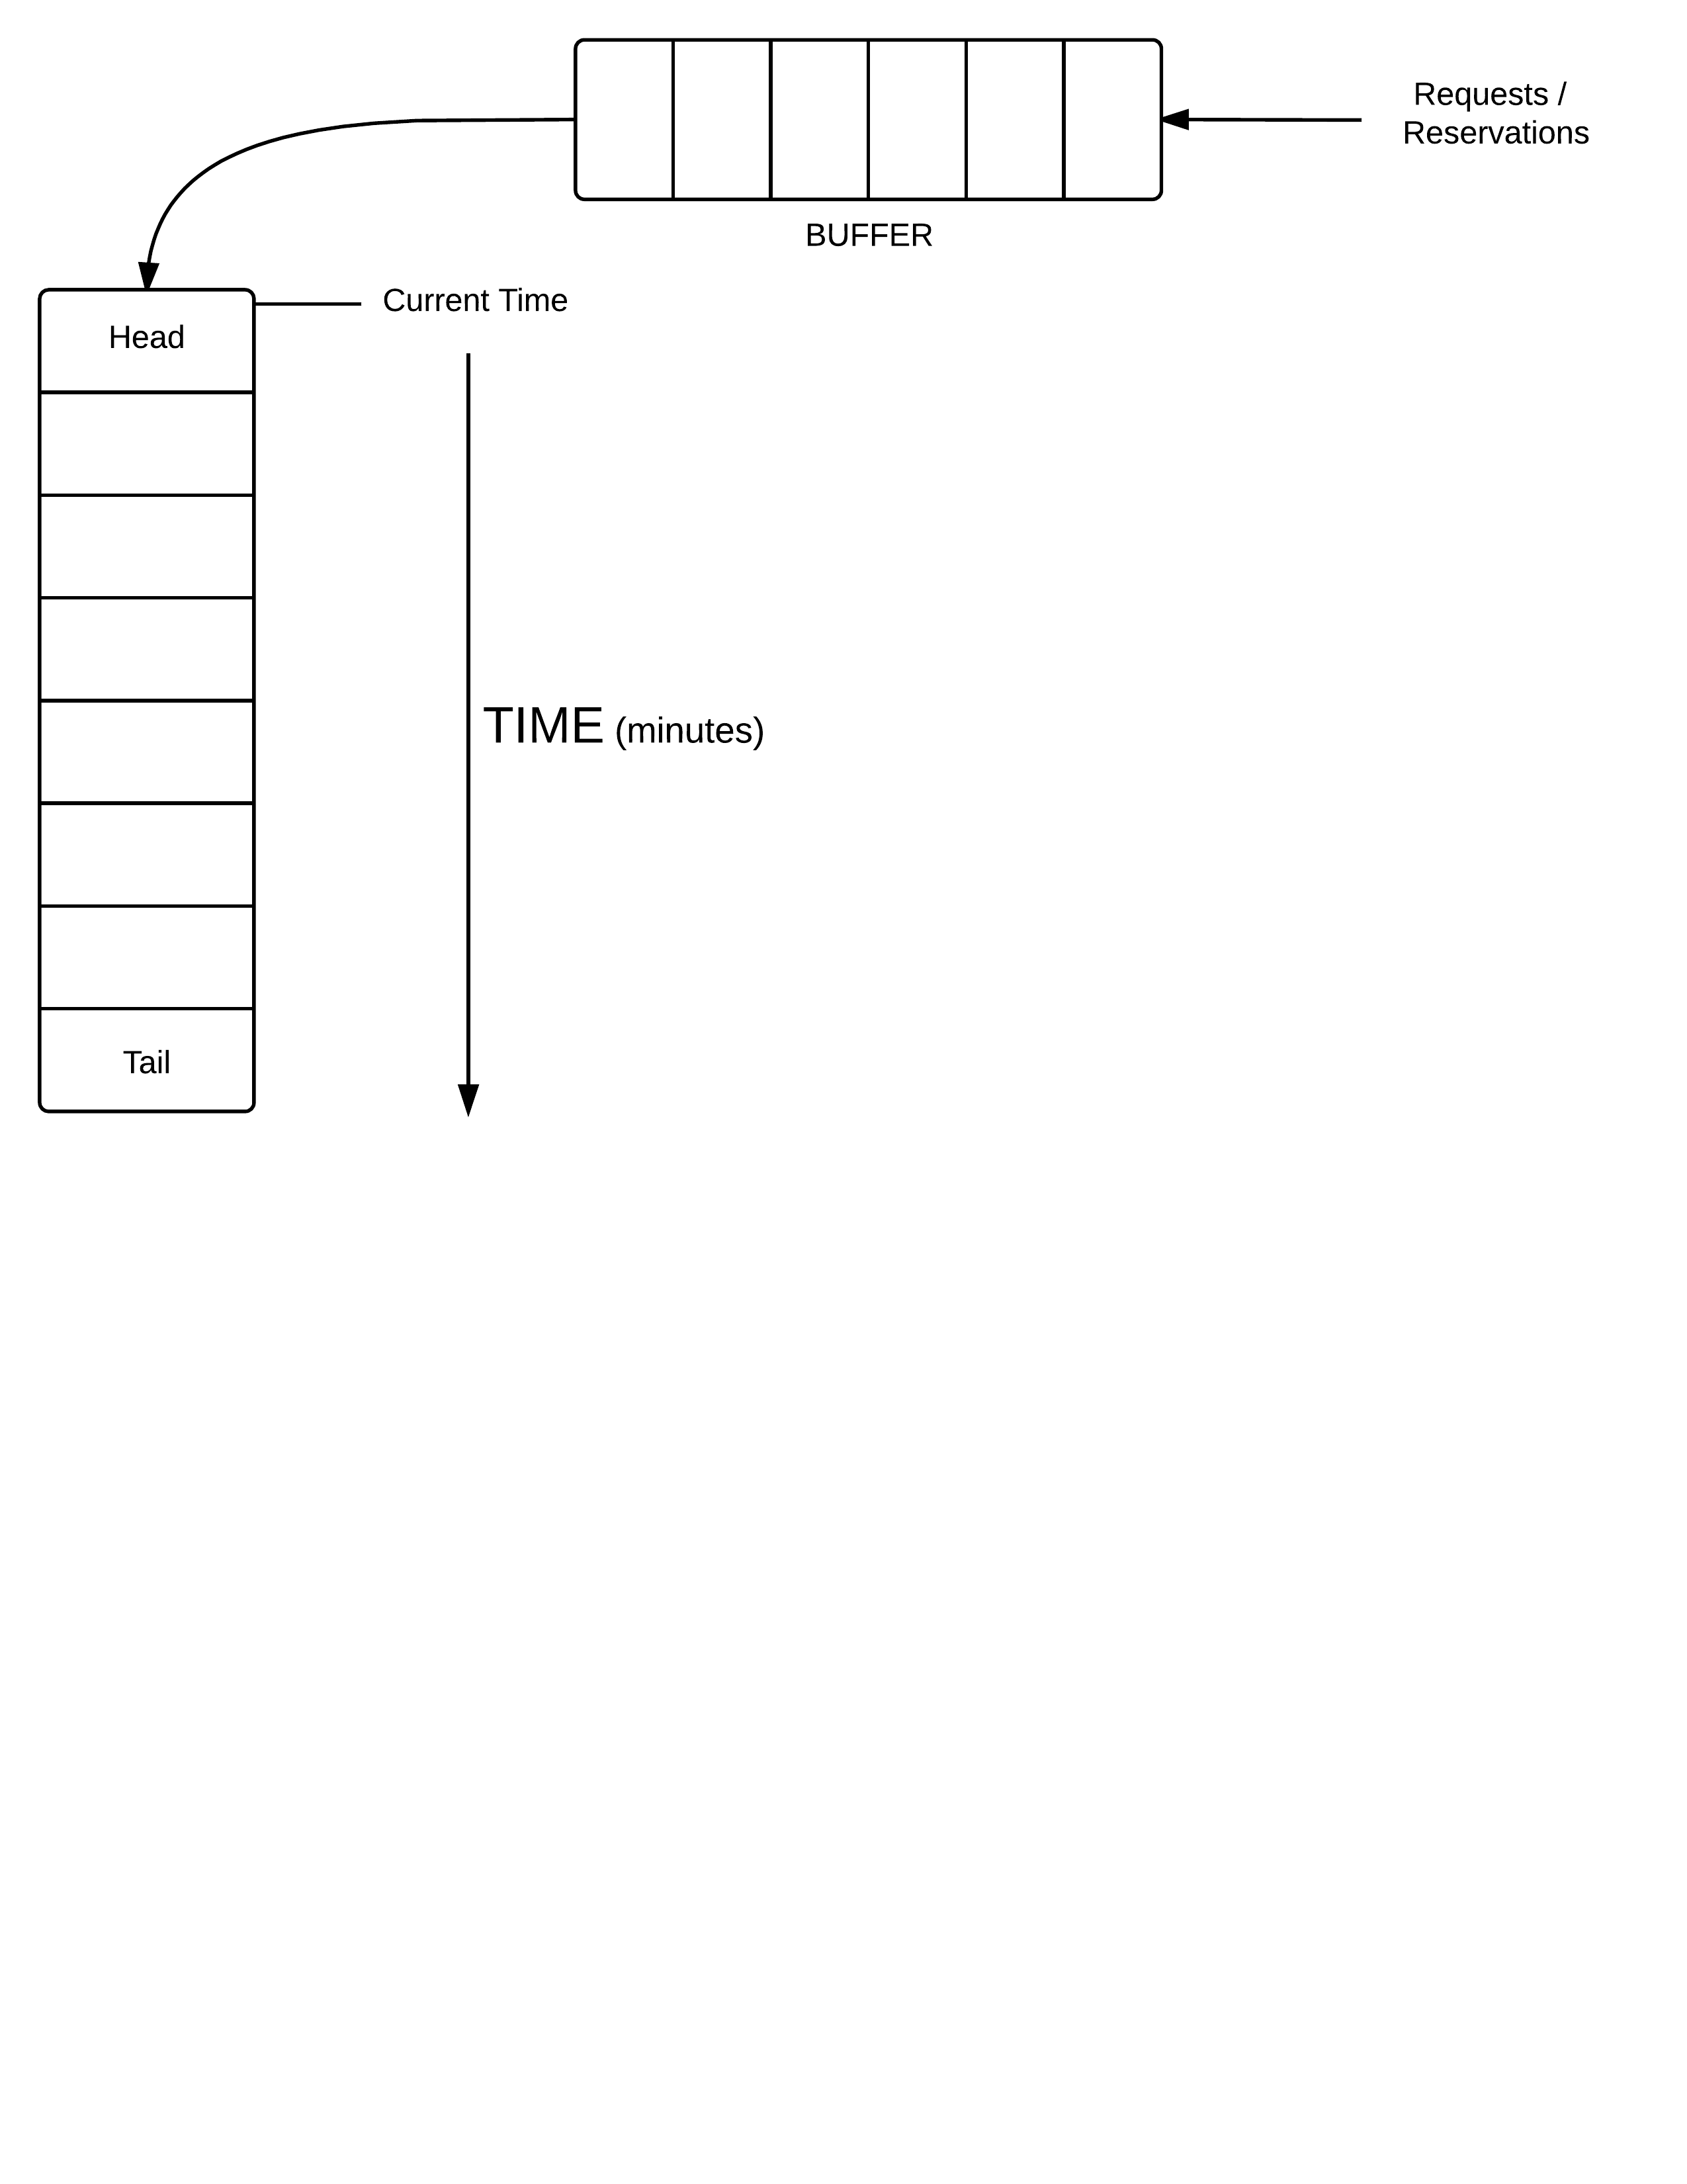
\includegraphics[width=\textwidth]{cpt/img/BufferQueue}
\caption{Representation of interaction between Queue and Buffer}
\label{fig:buff}
\end{figure}
\clearpage

\begin{figure}[htbp]
\centering
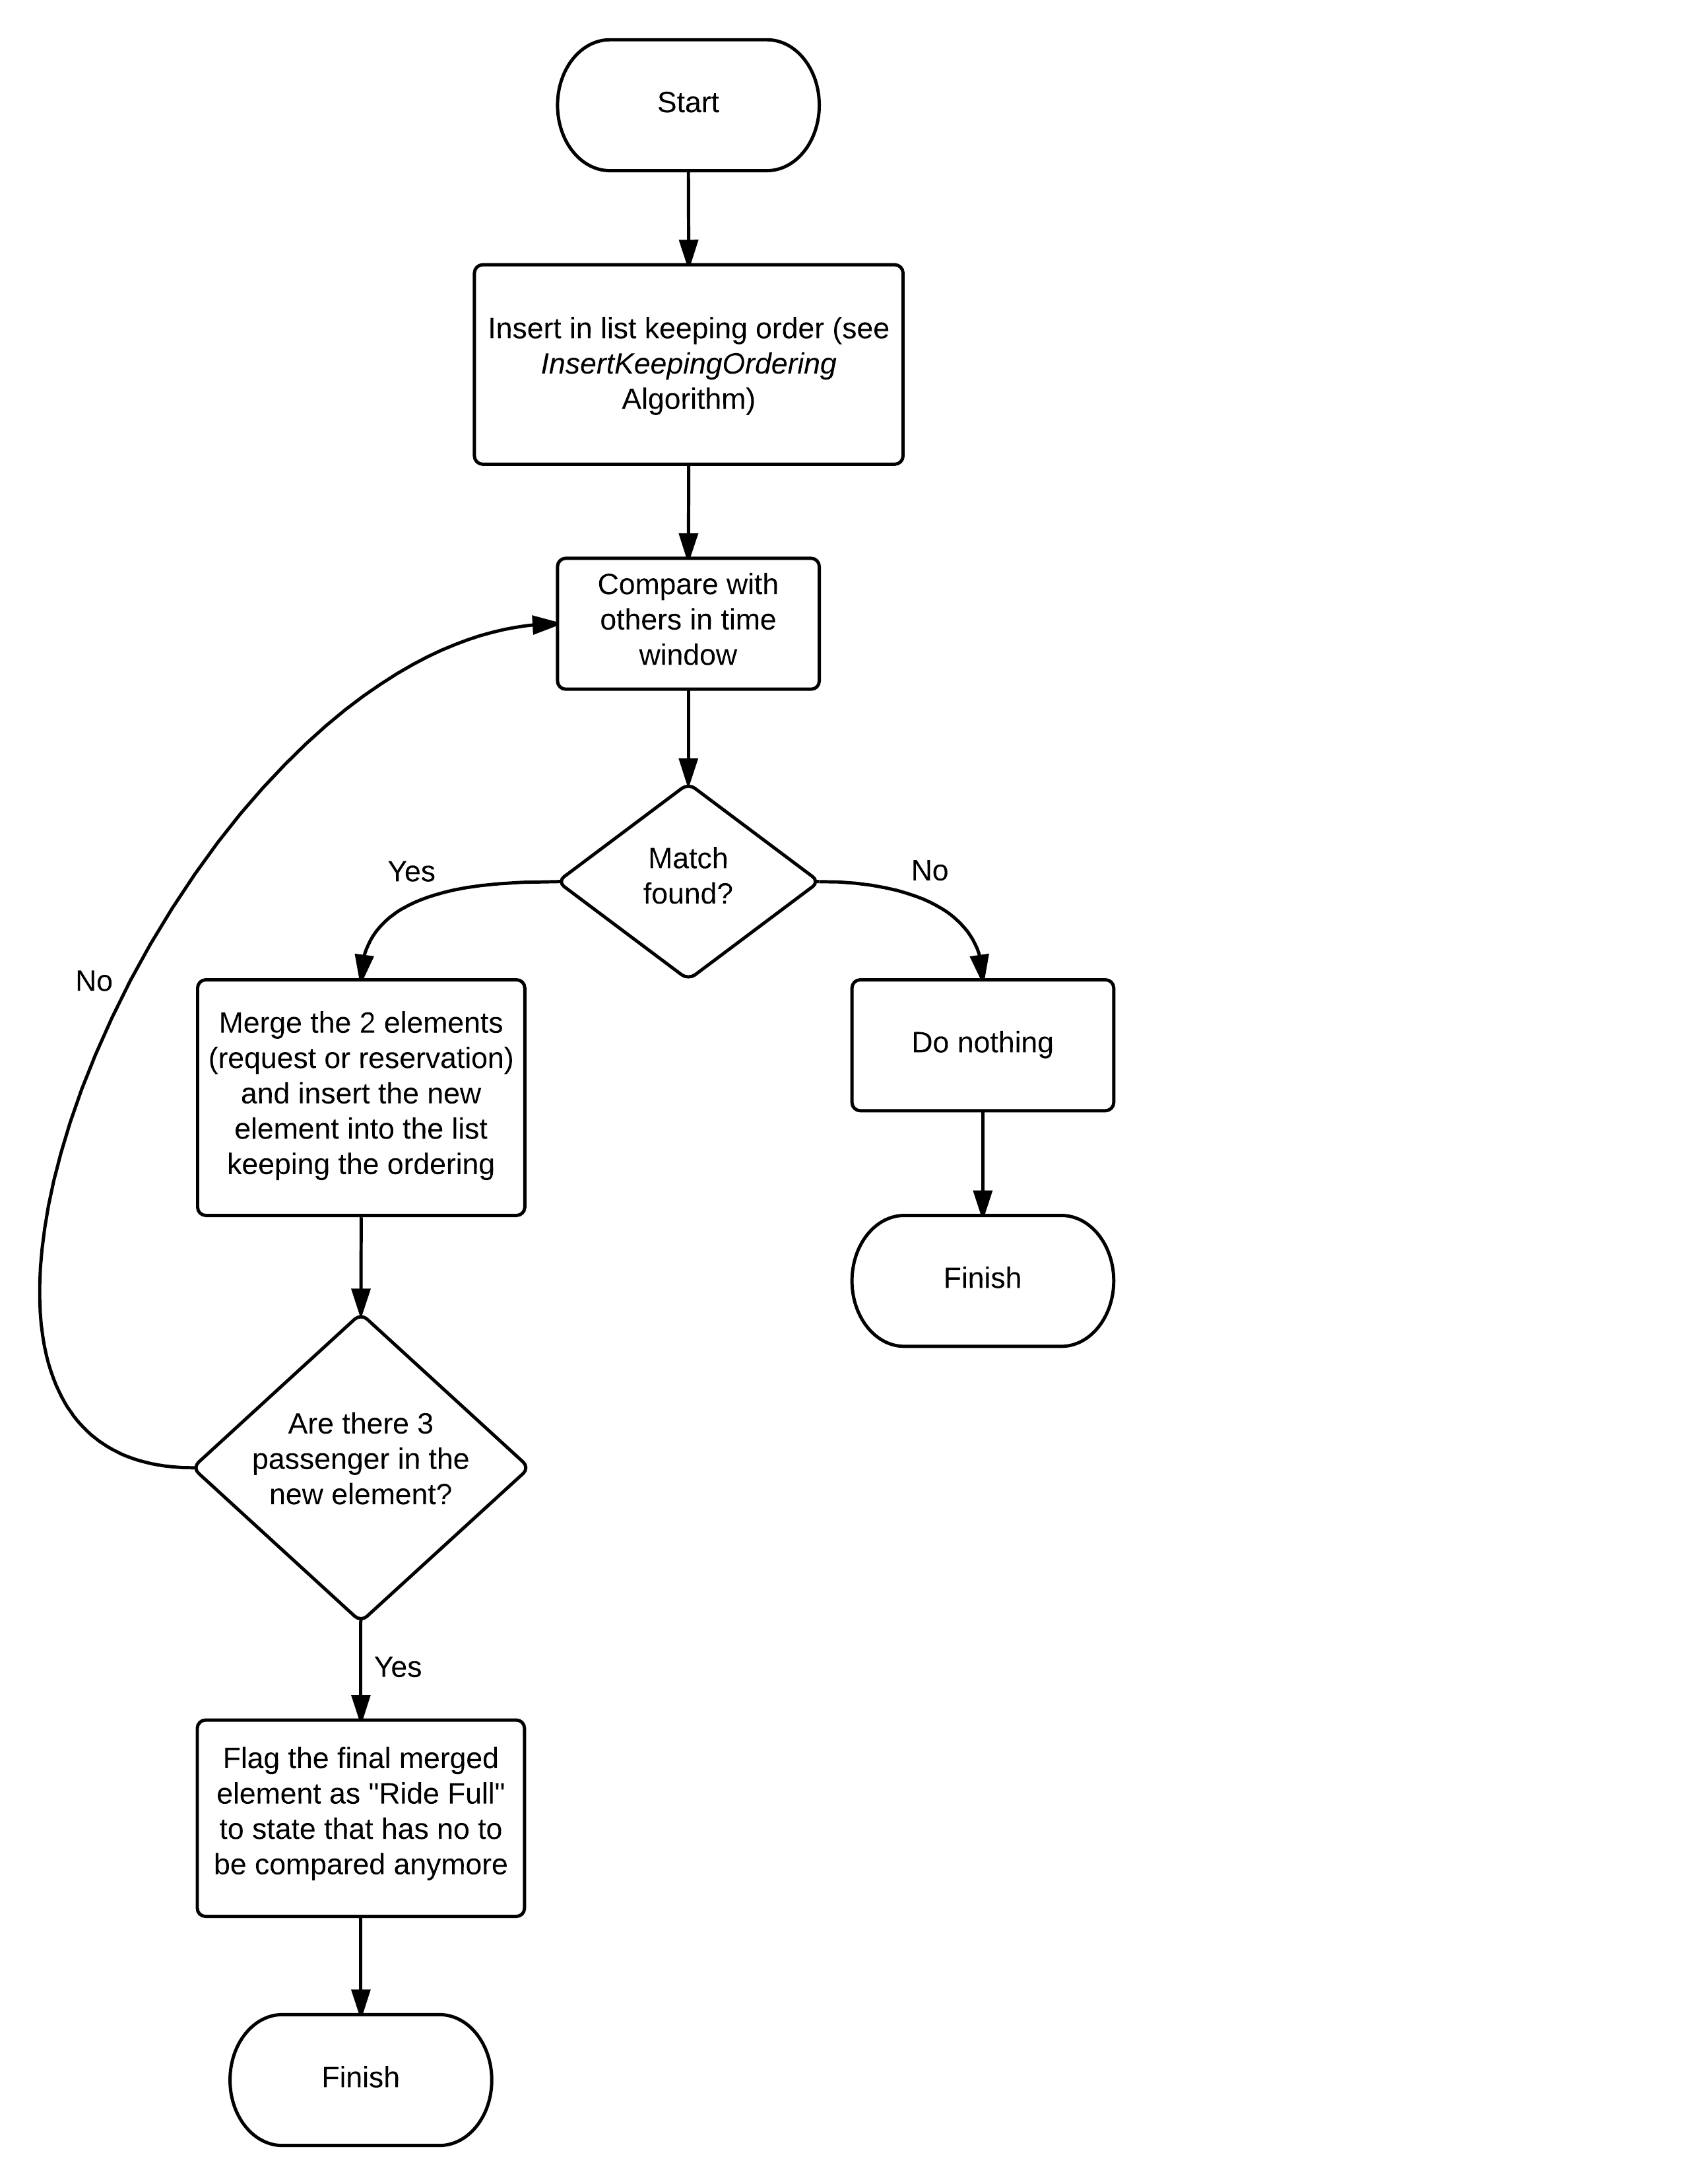
\includegraphics[width=\textwidth]{cpt/img/GenericAlgorithm}
\caption{Representation of the Shared Ride Management Algorithm}
\label{fig:genalg}
\end{figure}
\clearpage

The following algorithms describe in details the behavior of the list and how the Shared Ride Management Algorithm works:

\begin{algorithm}[H]
\caption{Check for Compatibility}
\begin{algorithmic}[1]
\Procedure{CheckForCompatibility}{$x, List$}
\For{$each \: element \: e \: \textbf{in} \: Sublist(x)$}\Comment{\textit{Sublist(x)} indicates the portion of the list starting from the successor of element \textit{x}}
	\If{$((e.startTime \leq x.startTime + 10)$ \textbf{\&\&} $(e.destinationArea == x.DestinationArea)$ \textbf{\&\&} $(e.flagAsFullRide == false))$}
		\State $\textit{MergeRides(x, e)}$
		\State ${\textbf{break()}}$
	\EndIf
\EndFor
\EndProcedure
\end{algorithmic}
\end{algorithm}

\begin{algorithm}[H]
\caption{Merge Rides}
\begin{algorithmic}[1]
\Procedure{MergeRides}{$x, y$}
\State \textit{Creates a new element z with the same originArea and destinationArea of x and y}
\If{$x.startTime < y.startTime$}
	\State $z.startTime \gets x.startTime$
	\Else
	\State $z.startTime \gets y.startTime$
\EndIf
\State \textit{All the other information about the request/reservation are copied from x and y into z}
\EndProcedure
\end{algorithmic}
\end{algorithm}

\begin{algorithm}[H]
\caption{Insert an element in List keeping the order}
\begin{algorithmic}[1]
\Procedure{InsertKeepengOrder}{$x, List$}
\For{$each \: element \: e \: \textbf{in} \: List$}
	\If{$(e.startTime \geq x.startTime)$}
		\State $e.prev.next \gets x$\Comment{\textit{e.prev.next} indicates the attribute next of the element pointed by \textit{e.prev}}
		\State $x.prev. \gets e.prev$
		\State $x.next \gets e$
		\State $e.prev \gets x$
		\State ${\textbf{break()}}$
	\EndIf
\EndFor
\EndProcedure
\end{algorithmic}
\end{algorithm}
\clearpage

\chapter{User Interface Design} \label{chap4}
Here are presented the UX Diagrams for the User Interface of both the Passengers and Taxi Drivers applications. Ux Diagrams are meant to show a detailed schema about the web site navigation done by the users of the system. For the complete mockups refer to the RASD document.

\begin{figure}[htbp]
\centering
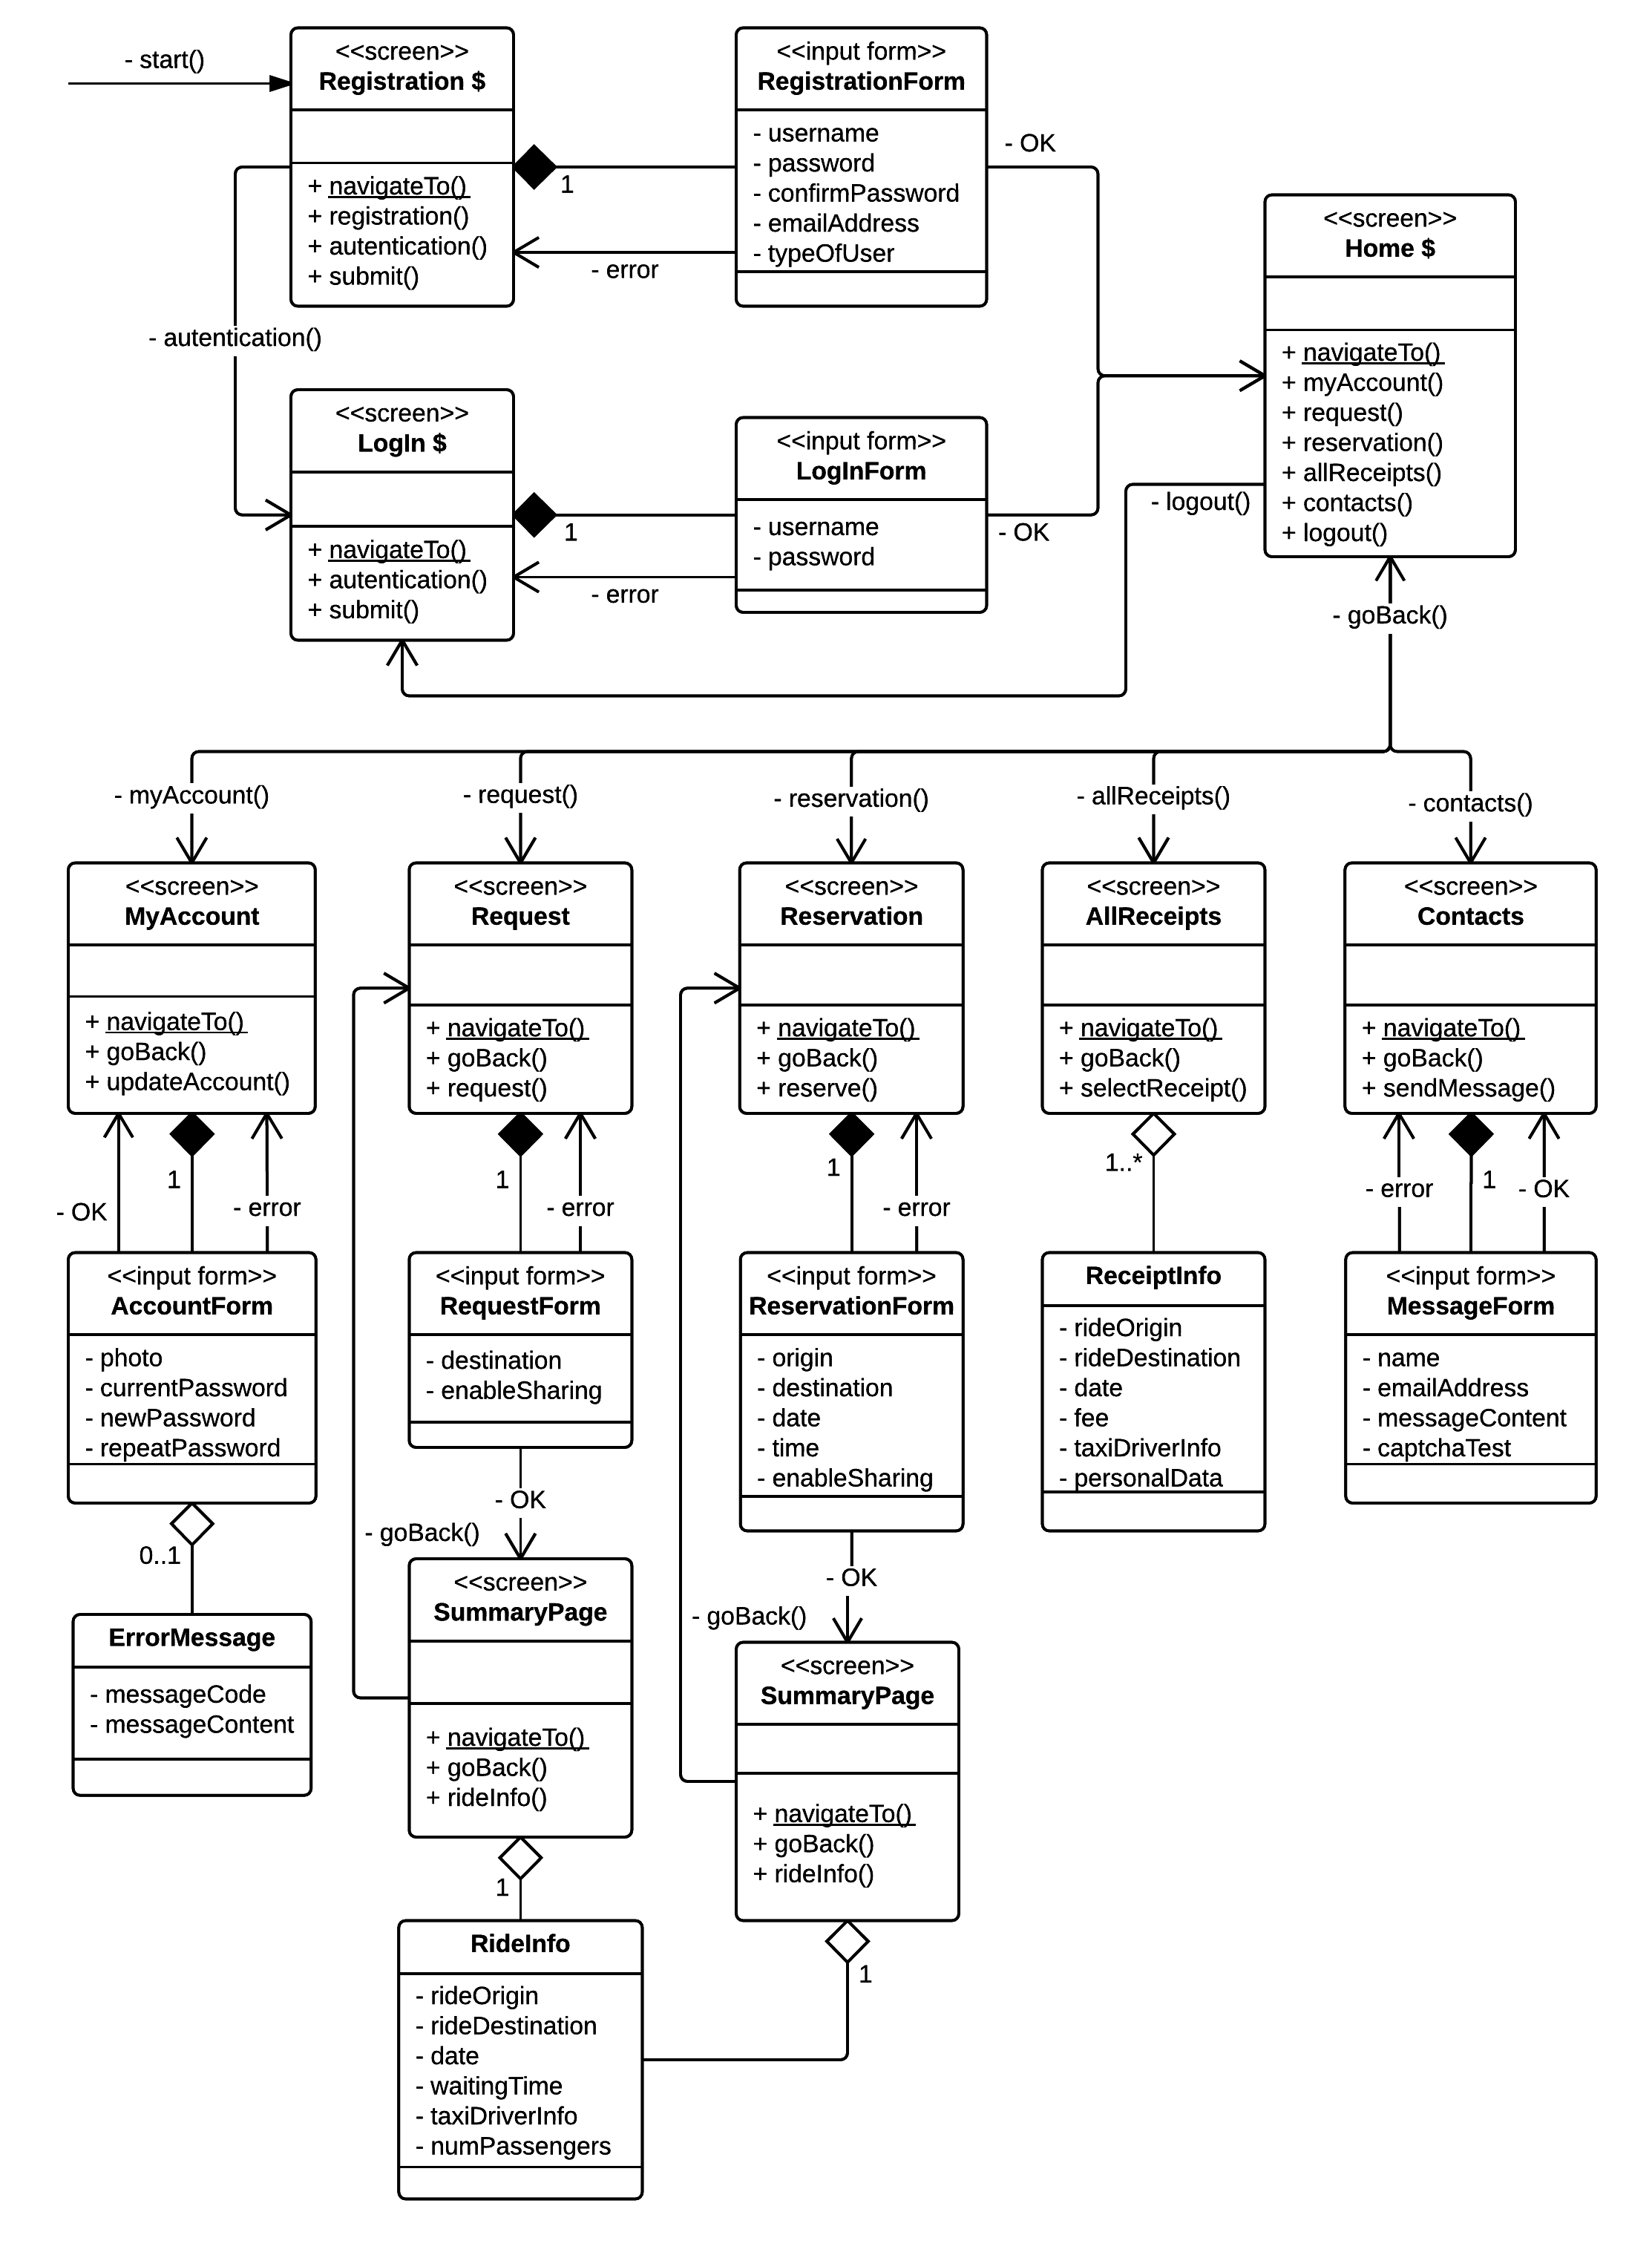
\includegraphics[width=\textwidth]{cpt/img/UXPassengerApp}
\caption{UX Diagram - Passenger Application Interface}
\end{figure}
\clearpage

\begin{figure}[htbp]
\centering
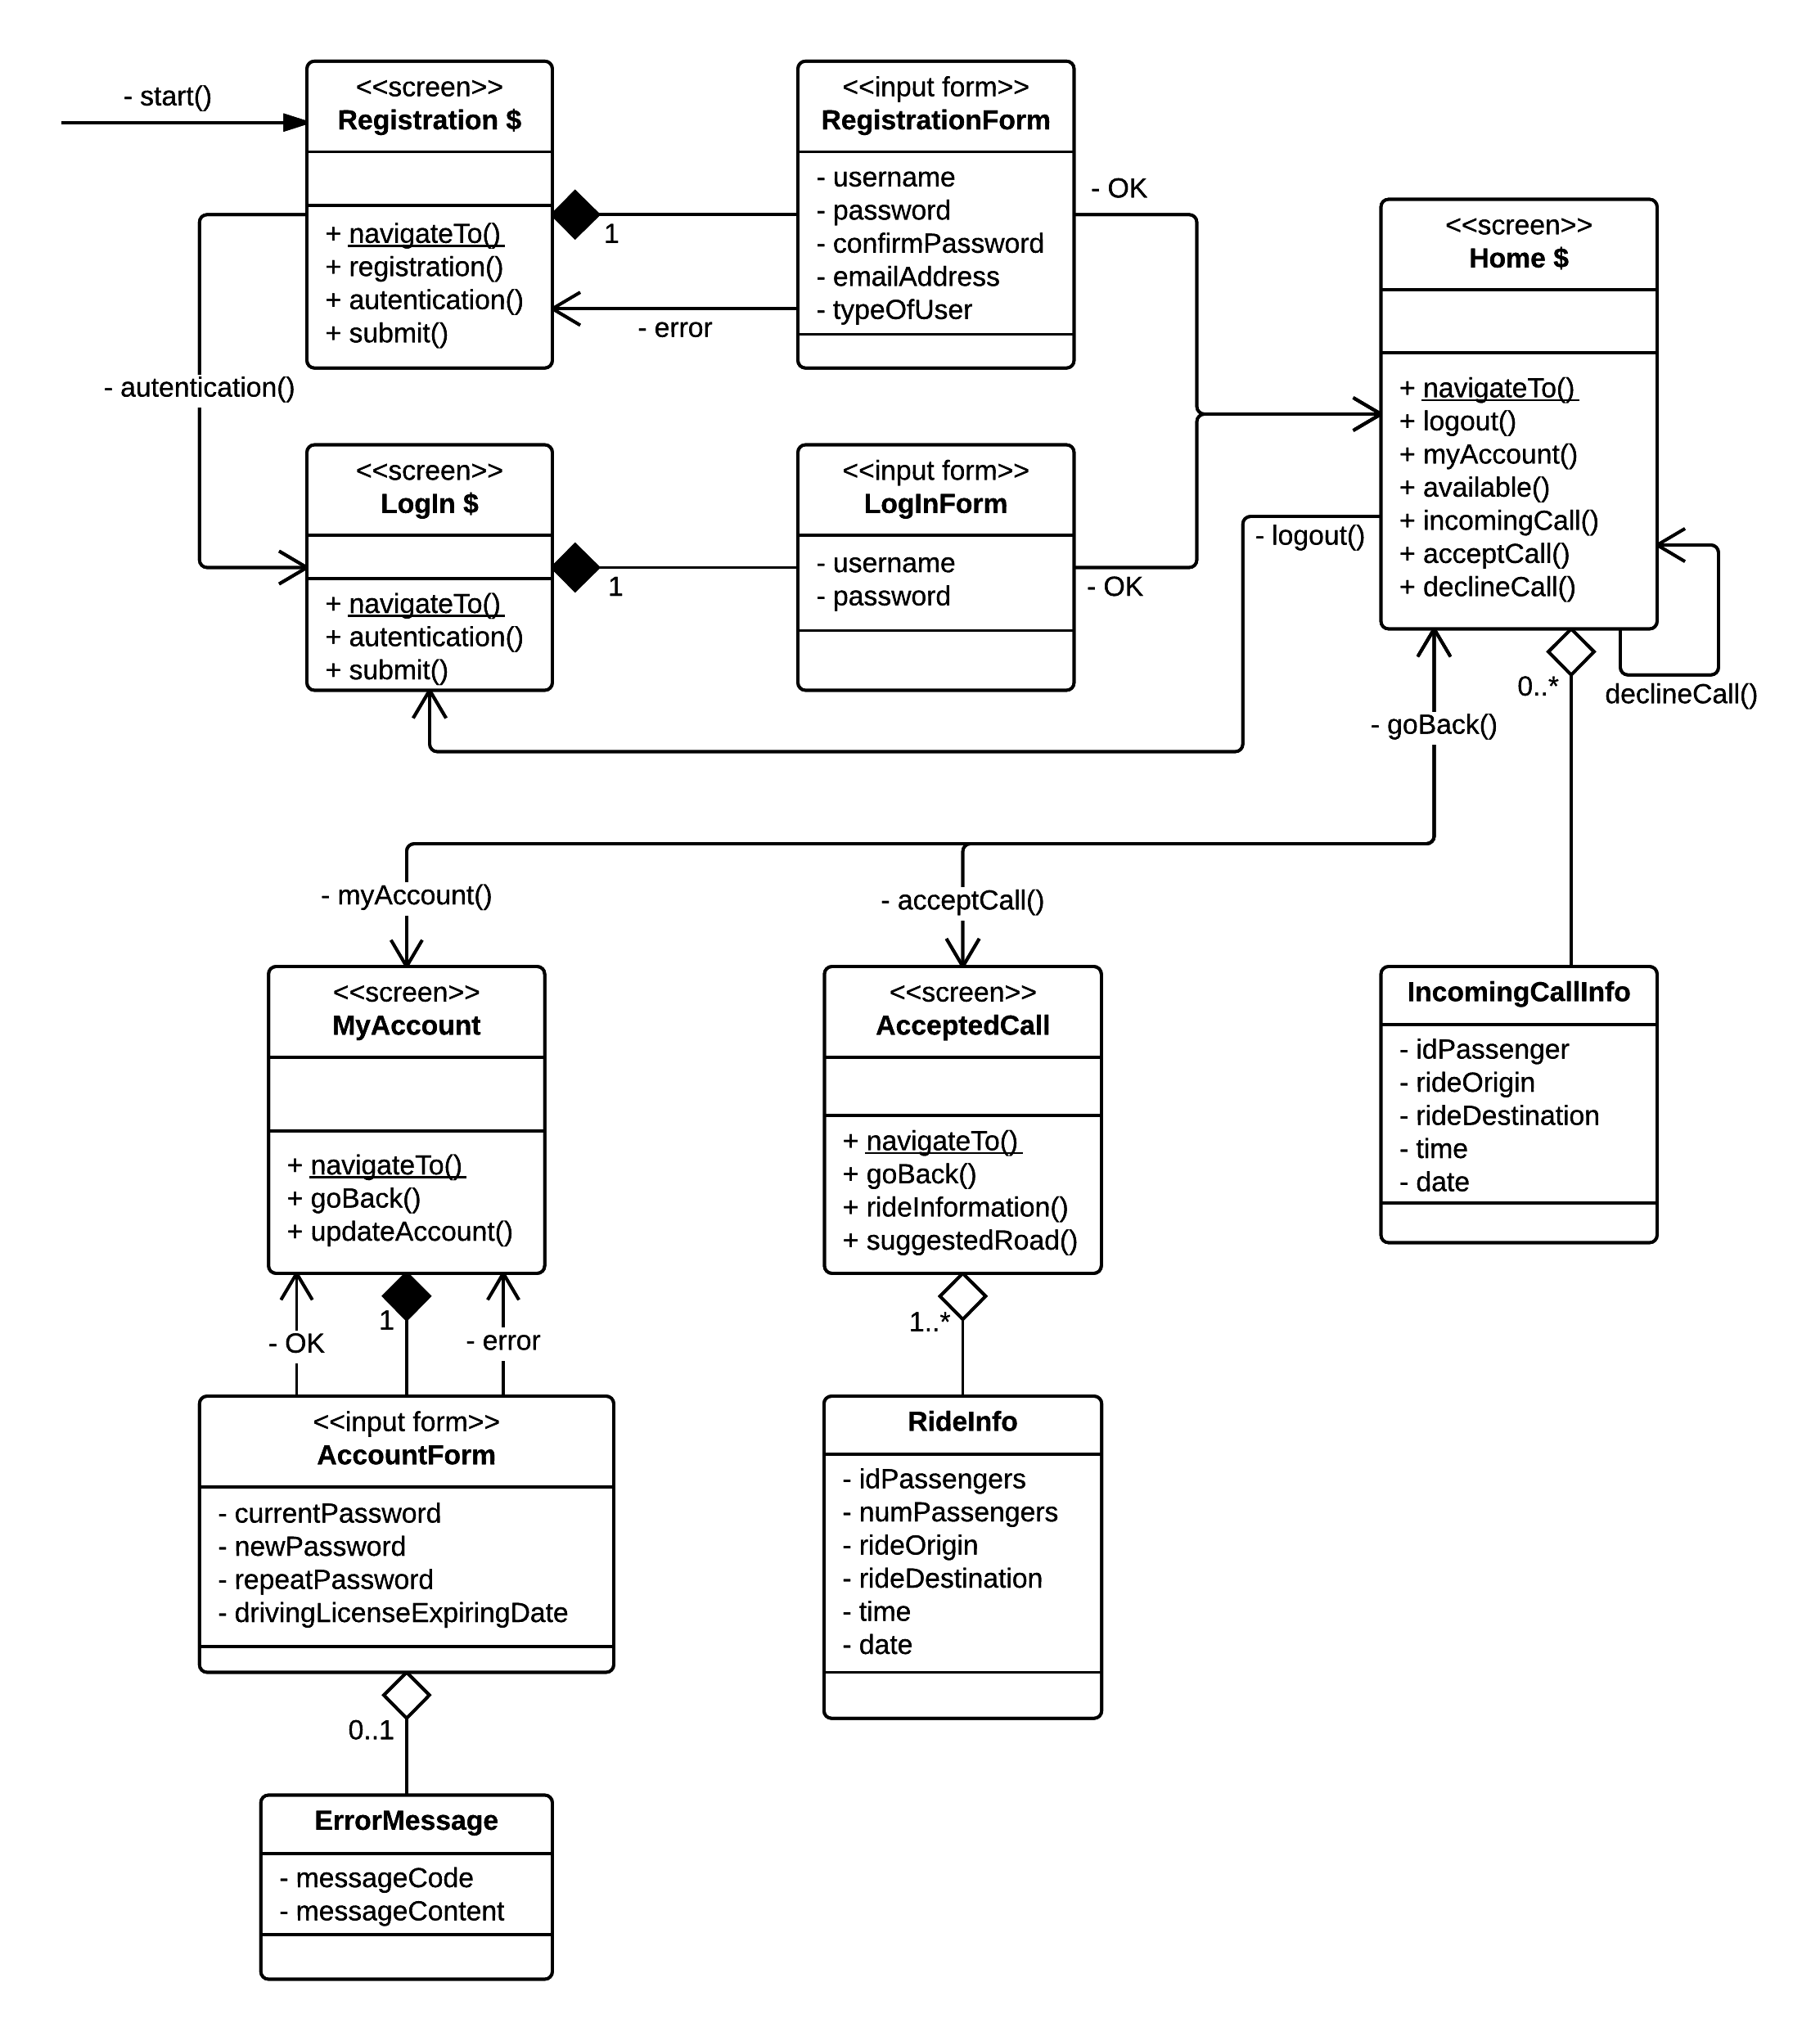
\includegraphics[width=\textwidth]{cpt/img/UXTaxiDriverApp}
\caption{UX Diagram - Taxi Driver Application Interface}
\end{figure}
\clearpage
\clearpage

\chapter{Requirements Traceability} \label{chap5}
\begin{itemize}
	\item [\textbf{R01}] check the validity and correctness of the information provided by the visitor (personal information, password)
	\begin{itemize}
		\item This requirement is satisfied by the validity and correctness controls inside the Visitor Manager
	\end{itemize}

	\item [\textbf{R02}] check if the user is already registered into the system
	\item [\textbf{R03}] check if username and password provided by the visitor correspond to an existing user, authorized to use the system
	\item [\textbf{R04}] prevent unauthorized or banned users from accessing the system
	\begin{itemize}
		\item These requirements are satisfied by allowing the Visitor Manager to query the Database
	\end{itemize}
	
	\item [\textbf{R05}] obtain the passenger location
	\begin{itemize}
		\item This requirement is satisfied in a Request by retrieving data from the GPS embedded in the passenger's smartphone and in a Reservation by allowing the Passenger to manually insert through the application interface his/her location (refer to UX Diagram - Passenger Application Interface)
	\end{itemize}

	\item [\textbf{R06}] access the queue associated to the right taxi zone
	\item [\textbf{R07}] check the availability of the taxi drivers 
	\item [\textbf{R08}] iteratively contact all the taxi drivers of the queue starting from the first one until one of them accepts the call
	\item [\textbf{R09}] iteratively search for an available taxi driver inside adjacent zones in the case that the right zone has an empty queue or all the contacted taxi drivers had declined the request
	\begin{itemize}
		\item These requirements are satisfied within the algorithm "Research of a Taxi Driver in the queue zone or in an adjacent queue zone"
	\end{itemize}

	\item [\textbf{R10}] obtain the taxi driver position and estimate the time needed by the taxi driver to reach the passenger
	\begin{itemize}
		\item This requirement is satisfied by retrieving data from the taxicab GPS locator 
	\end{itemize}
	
	\item [\textbf{R11}] obtain the taxicab unique identifier from the taxi drivers database
	\begin{itemize}
		\item This requirement is satisfied by allowing the Ride Manager to query the Database
	\end{itemize}
	
	\item [\textbf{R12}] check for each request or reservation if the passenger had selected the sharing function
	\item [\textbf{R13}] compare routes that start from the same taxi zone and determine whether or not they can be merged into one, according to specific rules of comparison
	\item [\textbf{R15}] elaborate an optimal route for taking every passenger to the right destination and show it to the taxi driver
	\begin{itemize}
		\item These requirements are satisfied within the algorithm "Shared Ride Management"
	\end{itemize}
	
	\item [\textbf{R14}] calculate the correct distribution of the fee according to specific rules based on the percentage of the kilometers shared with others or traveled alone
	\begin{itemize}
		\item This requirement is satisfied within the algorithm "Fee Calculation Function"
	\end{itemize}
	
	\item [\textbf{R16}] keep track of the actual route followed by the taxi driver and keep track of the actual duration of the ride
	\begin{itemize}
		\item This requirement is satisfied by retrieving data from the taxicab GPS locator
	\end{itemize}
	
	\item [\textbf{R17}] update the database information for each user
	\begin{itemize}
		\item This requirement is satisfied by allowing the Passenger Manager and the Taxi Driver Manager to query and update the Database and by allowing the users to insert through the application interface the new data (refer to UX Diagram - Passenger Application Interface and UX Diagram - Taxi Driver Application Interface)
	\end{itemize}

	\item [\textbf{R18}] monitor and collect inputs from taxi drivers
	\begin{itemize}
		\item This requirement is satisfied by allowing Taxi Drivers to interact with the system through an appropriate application interface (refer to UX Diagram - Taxi Driver Application Interface)
	\end{itemize}

	\item [\textbf{R19}] contact taxi drivers and forward them all the information about the proposed request (position of the passenger, destination of the passenger, sharing option enabled or not)
	\item [\textbf{R20}] retrieve the taxi location and the locations of all the passengers of the ride
	\begin{itemize}
		\item This requirement is satisfied within the algorithm "Research of a Taxi Driver in the queue zone or in an adjacent queue zone"
	\end{itemize}
	
	\item [\textbf{R21}] Access and query the map provider service to obtain an updated map with information about traffic, smashes, road construction sites
	\begin{itemize}
		\item This requirement is satisfied by exploiting the Google Maps API
	\end{itemize}
	
	\item [\textbf{R22}] Update the system code and architecture
	\begin{itemize}
		\item MANCA QUESTO
	\end{itemize}
\end{itemize}
\clearpage

\chapter{References} \label{chap6}
\section{External References}
Link referenced to documentation about JEE architecture:\\
\href{http://docs.oracle.com/javaee/6/tutorial/doc/bnaay.html} {http://docs.oracle.com/javaee/6/tutorial/doc/bnaay.html} \\ \\
Link referenced to documentation about the Java Interface Queue:\\
\href{http://docs.oracle.com/javase/7/docs/api/java/util/Queue.html} {http://docs.oracle.com/javase/7/docs/api/java/util/Queue.html} \\ \\
Link referenced to documentation about modeling:\\
\href{http://www.agilemodeling.com} {http://www.agilemodeling.com} \\ \\
Book referenced to documentation about algorithms:\\
Book ?Introductions to algorithms? by Cormen, Leiserson, Rivest, Stein - MIT Press (3rd edition)

\section{RASD Modifications}
\subsubsection{New Domain Properties:}
\begin{itemize}
	\item {[D01]} Taxicabs are all equals. They have a maximum of 3 passenger seats and they are all owned by a specific company.
	\item {[D02]} Every taxi driver uses always the same taxicab
	\item {[D09]} The total fee of a ride is calculated considering only the total kilometers of the ride, given a specific fee per km
\end{itemize}

\subsubsection{Changes in Functional Requirements:}
\begin{itemize}
	\item {[R10]} obtain the taxi driver position and estimate the time needed by the taxi driver to reach the passenger
\end{itemize}

\subsubsection{Add new functionality "Update Account":}
\begin{itemize}
	\item add new use case "Update Account" and its description
	\item add new functional requirement [R17]
	\item add new goals [G08] and [G13]
	\item mockup modification for the Passenger Home Page and Taxi Driver Home Page
add new states in the State Chart Diagram for Passengers and State Chart Diagram for Taxi Drivers
\end{itemize}

\section{Working Hours}

\begin{table}[htbp]
\begin{center}
\begin{tabular}[t]{ccc}

\hline
\textbf{First Name} & \textbf{Last Name} & \textbf{Total Hours} \\
\hline
Mattia & Crippa &  23h\\
\hline
Francesca & Galluzzi &  25h\\
\hline
Marco & Lattarulo & 26h\\
\hline

\end{tabular}
\end{center}
\end{table}

\clearpage

\end{document}
